% !TeX root = ../thesis.tex
\chapter{Overview\label{chapter:1}}

\begin{chaptersections}{%
We introduce Bayesian nonparametric glottal inverse filtering (BNGIF) and provide a high-level overview of the main concepts involved, followed by a summary of the contributions made in this thesis.
}

\section{Introduction\label{sec:introduction}}

In this thesis we present a new approach to the problem of \emph{glottal inverse filtering} (GIF) called \emph{Bayesian nonparametric glottal inverse filtering} (BNGIF).
At the heart of this new approach lies a Bayesian nonparametric \emph{generative model of voiced speech} that reflects general constraints on the voice production process.
Though conceived for GIF, the generative model can be conditioned on both raw speech data and high level speech features, which makes it useful for other related tasks such as augmenting or denoising speech data.
%This generative model reflects several general constraints on the voice production process and can be conditioned on raw speech data and speech features.
%These properties lend the model a generality that makes it useful for a variety of tasks other than GIF, though our primary application in this thesis is of course BNGIF.

Speech can be thought of as the output of a linear system in which an upstream source signal (for example, the rapid opening and closing of the vocal folds) is modulated by a downstream filter (for example, the oral cavity and lips).
This linear approximation to speech production, called source-filter theory \citep{Fant1960}, still underlies most of what is known today as acoustic phonetics \citep{Maurer2016}, and both source and filter are comparably well understood.

The GIF problem refers to source-filter separation of speech; that is, simultaneously inferring both the glottal source signal and (some of) the vocal tract filter characteristics from the speech signal alone (Figure~\ref{fig:source-filter-overview}).
In the BNGIF approach we systematically take advantage of known constraints on the voice production process to home in on scientifically plausible solutions to the GIF problem.
That is the main theme of this thesis.

\centeredfigure{test}{%
Bayesian nonparametric glottal inverse filtering (BNGIF).
}{%
\shloppy{%
% img/mypaint-test.pnsg
The speech waveform (left) is modeled as a glottal source signal (top right) passing through a series of vocal tract filters (bottom left).
The task is to find such plausible source-filter pairs (colored samples on the right) that together produce a given speech waveform.
}
}

GIF is an important and difficult problem in acoustic phonetics \citep{Auvinen2014,Kadiri2021} and various approaches have been developed over the last 60 years.
Paraphrasing \cite{Alku2011}, applications mainly come in three broad categories: (i) fundamental research about voice production (for example, quantifying voice quality), (ii) medical applications (such as analysis of pathological voices), and (iii) speech technology applications (for example, voice modification).
To this we would add (iv) recent forensic and biometric applications such as evidence-based speaker identification \citep{Bonastre2015}.

Our approach to the GIF problem is mostly relevant to the first category (i) above because we try to model the process of scientific inference -- make assumptions, model the data, fit the data, evaluate the model, reiterate -- as a whole rather than `just' modeling the data alone \citep[Ch.~28]{MacKay2005}.
It has been shown repeatedly that the unique way to do this is the probabilistic or \emph{Bayesian} framework \citep{Knuth2012}.
Within this mathematical framework our generative model of voiced speech ultimately expresses nothing more than our assumptions about voice production in a logically coherent way.
Because we insist on modeling scientific inference itself the accuracy of those assumptions will translate directly to the accuracy of our measurements, providing a much-needed means to calibrate uncertainty for use in (i) fundamental research about voice production \citep{Kent2018}.
This is the main benefit of and motivation for using the Bayesian framework for BNGIF, despite its considerable computational expense compared to standard GIF algorithms which are based on traditional signal processing methods.

Another important benefit is the standardized form of Bayesian generative models:
posterior inference is mechanical once the prior and likelihood are specified, which allows for a wide variety of generic algorithms to fit the data in true plug-and-play fashion \citep{Murphy2022}.
This standardized form also ensures that generative models are easily modifiable and extendable for more specific applications such as (ii-iv) mentioned above.\footnote{%
For example it is expected that our model of human voice production can be useful for mammal vocal communication research \citep{Taylor2010} by simply tweaking some of its prior assumptions.
An example of extending the model to downstream tasks is forensic phonetics, since ``formant features [...] are widely accepted features used in forensic acoustic-phonetic speaker verification'' \citep[][p.~1]{Becker2008} and ``the Bayesian decision framework [...] is now the standard paradigm for forensic speaker comparison'' \citep[][p.~1]{Bonastre2015}.
This Bayesian decision framework depends on likelihood ratios \citep{Harrison2013} that can be calculated with the same computational tools used in this thesis.
}

Another distinguishing feature of BNGIF is the \emph{nonparametric} nature of our generative model of speech.
More precisely, the model contains both nonparametric and parametric components.
Figure~\ref{fig:source-filter-overview} shows these two neatly divided components on the right hand side:
the glottal source signal (top) is modeled nonparametrically with a Gaussian process \citep[GP;][]{Rasmussen2006}, while the vocal tract filter (bottom) is expanded into a familiar rational transfer function that is parameterized by an overall gain factor and a vector of poles and zeros.

Nonparametric in this context does not refer to `distribution-free' methods used in descriptive statistics or nonparametric spectral analysis \citep{Stoica2005};
rather it means that the glottal source signal is modeled directly through an infinite-dimensional distribution over functions whose qualitative behavior is specified by a just few global properties like roughness and wiggliness.
This is convenient because this is exactly the kind of broad information we possess about the glottal source signal, unlike the vocal tract filter which in source-filter theory is naturally specified in terms of resonances of the vocal tract \citep{Stevens2000}.

% Insert PDF figure here at path: 
\begin{figure}
\centering
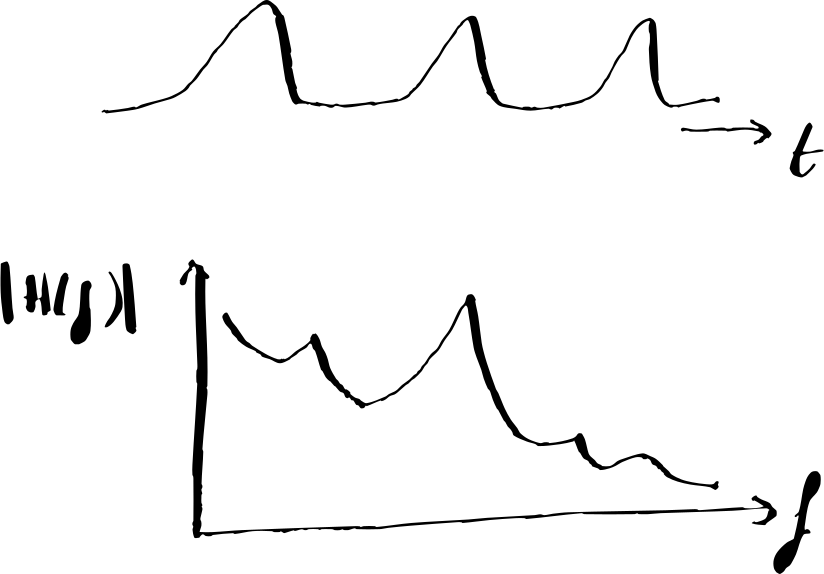
\includegraphics[width=\textwidth]{/home/marnix/thesis/figures/notebooks/iklp/test.pdf}
\end{figure}

%This concludes our high-level overview of this thesis.
%In the next section we describe the source-filter separation problem in more detail before motivating our approach.

\section{Problem statement\label{sec:problem-statement}}

The central problem of this thesis can be stated as follows:

\begin{mdframed}[frametitle={Glottal inverse filtering (GIF)}]
Assume that the source-filter model of speech production \citep{Fant1960} holds such that the speech signal at time $t \in \mathbb{R}$ is described by convolving three real-valued functions: 
\begin{equation}
    s(t) = u(t) * h(t) * r(t). \label{eq:lti-full}
\end{equation}
From left to right $s(t)$ is the speech pressure waveform, $u(t)$ is the glottal flow waveform, $h(t)$ is the impulse response of the vocal tract and $r(t)$ is the impulse response of the radiation characteristic, assumed known.
Source-filter theory asserts that $s(t)$ can be thought of as the result of the source signal $u(t)$ passing through the filters $h(t)$ and $r(t)$.

The data consists of $N$ noisy samples $\bd = d_{1:N}$ of the speech pressure waveform $s(t)$ at times $\bt = t_{1:N}$.
We assume additive errors $\be = e_{1:N}$ such that
\begin{align} 
\bd &= \bs + \be \\
\Longleftrightarrow \quad d_n &= s(t_n) + e_n \quad (n = 1 \cdots N).
\end{align}
The error components $e_n$ are modeled as white noise with expected power $\sigma_n^2$ which means that $e_n  \sim \Normal(0, \sigma_n^2)$ for $n = 1 \cdots N$.

The data $(\bt,\bd)$ is possibly augmented with noisy statistics of $s(t)$ such as a list of estimated glottal closing instants (GCIs).

% ``The estimation of the glottal source waveform by GIF is based on estimating the vocal tract filter'' (Kadiri 2021)
The GIF problem is then to \emph{find plausible estimates of the source $u(t)$ and the filter $h(t)$} that are consistent with the given data.
\end{mdframed}

Source-filter theory as expressed by equation \eqref{eq:lti-full} is the most important assumption in this thesis because it provides a definite handle on the GIF problem.
Even just stating the problem would be difficult without it.
In particular, note the four functions (or waveforms) in \eqref{eq:lti-full}:
each of these play an important role in BNGIF.
Before reviewing them in Section~\ref{sec:source-filter-theory}, we first consider how the \emph{plausible estimates} mentioned in the statement above translate within the Bayesian framework adopted in this thesis.

%We can now be a bit more precise with regard to the main theme of this thesis as stated in Section~\ref{sec:introduction}.
Like most inverse problems, the main difficulty with GIF lies in the fact that it is vastly underdetermined: even in the noiseless case ($\bd = \bs$), many solutions (that is, pairs of functions $u(t)$ and $h(t)$) are compatible with given data $\bd$ \citep{Landau1983}.
It thus appears that next to the data $\bd$ itself we need additional criteria to choose between possible solutions of \eqref{eq:lti-full}, and this is where the idea of regularization comes in.

Appendix~\ref{app:regularization} discusses how in the Bayesian framework regularization is imposed by assigning priors to the unknown functions $u(t)$ and $h(t)$ in such a way that these priors express known constraints on the voice production process.
The main idea is that a probability in the Bayesian framework describes a state of knowledge, not necessarily related to an observed frequency in the real world, so we can conveniently use prior probabilities to express constraints on the voice production process.

Even with that regularization in place, we will see that the problem is still underdetermined in the sense that we cannot in general expect to find unique solutions: the best we can hope for are \emph{plausible estimates in the form of posterior samples of $u(t)$ and $h(t)$}.
These are plausible in the sense that they are consistent with both the speech data $\bd$ and whatever prior information about voice production we have expressed through the priors for $u(t)$ and $h(t)$.

\section{Source-filter theory\label{sec:source-filter-theory}}

% \centeredfigure{source-filter-theory}{%
% Source-filter model of speech production.
% }{%
% \shloppy{%
% Schematical representation of the source-filter model \eqref{eq:lti-full} with $u,h,r,s$ and their Fourier transforms.
% }}

Source-filter theory\footnote{%
Currently the dominant paradigm in acoustic phonetics \citep{Maurer2016},
the source-filter theory of voice production is commonly attributed to \cite{Fant1960} but appears to date back to the early 19th century \citep{Chen2016}.
Its strength lies in its extremely useful and compact description of the acoustics of phonation, summarized by \cite[][p. 15]{Fant1960} as ``the speech wave is the response of the vocal tract filter systems to one or more sound sources.''
A modern perspective on source-filter theory is given by \cite{Svec2021}.
} models the speech production process as a standard \emph{linear time-invariant} (LTI) system \citep{Antsaklis2006} which is essentially a linear approximation to the underlying nonlinear dynamics of voice production that is roughly valid up to frequencies of 4 or 5~kHz \citep{Doval2006}.
The LTI system \eqref{eq:lti-full} used in this thesis is illustrated in Figure~\ref{fig:source-filter-theory}.
We proceed with a brief sketch of the important concepts involved.

The \emph{input} to the system is the source $u(t)$.
The system has two \emph{transfer functions} which determine how the amplitudes and phase of the frequencies present in the input $\utilde(x)$ are modified or filtered by the system to produce the \emph{output}.
That frequency decomposition
\begin{equation}
    \utilde(x) = \mathcal{F}\qty[u(t)](x) = \int_{-\infty}^\infty u(t) \exp{-i2\pi xt} \dd{t} \label{eq:ux}
\end{equation}
is obtained by the Fourier transform $\mathcal{F}$ of $u(t)$.
Note that the system's transfer functions is assumed to be independent from its input: source-filter theory assumes source and filter to be decoupled.

The vocal tract transfer function $\htilde(x)$ describes the resonances and antiresonances of the vocal tract (comprising the throat, mouth and nasal cavity), while the radiation characteristic $\rtilde(x)$ describes the lip radiation effect.
These transfer functions can be described equivalently in the time domain by the \emph{impulse responses}
\begin{align}
    h(t) &= \mathcal{F}^{-1}\qty[\htilde(x)](t) = \int_{-\infty}^\infty \htilde(x) \exp{i2\pi tx} \dd{x} \label{eq:ht} \\
    r(t) &= \mathcal{F}^{-1}\qty[\rtilde(x)](t) = \int_{-\infty}^\infty \rtilde(x) \exp{i2\pi tx} \dd{x} \label{eq:rt}
\end{align}
using the inverse Fourier transform $\mathcal{F}^{-1}$.
Unlike $u(t)$ and $h(t)$, $r(t)$ is assumed fixed and known: the lip radiation effect is modeled in the GIF literature as a standard 6 dB/octave high pass filter \cite[][p.~128]{Stevens2000} which has transfer function $\rtilde(x) = -i2\pi x$.
This corresponds to differentiation in the time domain as \eqref{eq:rt} yields $r(t) = \delta'(t)$.\footnote{%
Convolution of a test function $f(x)$ with the derivative of the Dirac delta function is equivalent to differentiation: $f(t) * \delta'(t) = f'(t)$.
This can be justified by considering nascent delta functions such as the Gaussian $\exp{-t^2/a^2}/\sqrt{2 \pi a^2}$ and then taking the limit $a \rightarrow 0$.
}

The output of the system is the speech pressure signal $s(t)$
\begin{align}
    s(t) &= u(t) * h(t) * r(t) &\text{(time domain)} \tag{\ref{eq:lti-full}} \\
    \Longleftrightarrow \quad \stilde(x) &= \utilde(x) \phantom{*} \htilde(x) \phantom{*} \rtilde(x) &\text{(frequency domain)} \label{eq:lti-x}
\end{align}
assumed to be measured in the free field (that is, sufficiently far from the speaker's head) \citep{Stevens2000}.
Filtering in LTI systems happens through multiplication in the frequency domain \eqref{eq:lti-x}, which is equivalent to convolution in the time domain \eqref{eq:lti-full}.

The meaning of these equations is best understood in the frequency domain.
During speech production, the source drives the air in the vocal tract such that it vibrates with some initial distribution over frequencies $\utilde(x)$.
Excited, the vocal tract filter $\htilde(x)$ reacts: frequencies in $\utilde(x)$ close to its resonance frequencies are emphasized,\footnote{%
The vocal tract filter is \emph{passive}, meaning that $|\htilde(x)| < 1$ for all frequencies $x$ \citep{Flanagan1965}.
The resonances of the vocal tract do not actively amplify frequencies;
frequencies close to the resonance frequencies are just less dampened relative to neighbouring frequency bands.
} while frequencies in $\utilde(x)$ close to its antiresonance frequencies are (often brutally) suppressed.
The result of this spectral imprinting is then radiated from the lips into the free field.
This radiation effect is contained within $\rtilde(x)$: high frequencies are emphasized, essentially because the lips act like small (passive) tweeters \citep{Schroeder1999}.
We are able to \emph{hear} the spectral imprint of the speaker's vocal tract on the initial energy distribution \citep{Klatt1986}, because it is what we use to tell the difference between different speech sounds, and ultimately to understand the speaker's message.
% Klatt in this paper shows that humans generally do not hear formants but the actual resonances. See Whalen (2022).

Since $r(t)$ is assumed known, we can further simplify \eqref{eq:lti-full} by substituting $r(t) = \delta'(t)$:
\begin{equation}
    s(t) = u(t) * h(t) * \delta'(t) = [u(t) * \delta'(t)] * h(t) = u(t) * [h(t) * \delta'(t)].
\end{equation}
We can differentiate either $u(t)$ or $h(t)$ in \eqref{eq:lti-full} because convolution is associative; we choose to differentiate $u(t)$ as is customary in the literature \citep{Doval2006}.
This finally yields
\begin{equation}
    \boxed{s(t) = u'(t) * h(t)} \label{eq:suh}
\end{equation}
where $u'(t)$ is the \emph{glottal flow derivative} (DGF) which now acts as the source driving the single filter in \eqref{eq:suh}.
The original source $u(t)$ can be recovered through integration:
\begin{equation}
    u(t) = \int_{-\infty}^t u'(\tau) \dd{\tau} \qq{with} u(-\infty) := 0. \label{eq:udu}
\end{equation}
Equation \eqref{eq:suh} is the basis for the nonparametric generative model of $s(t)$ which we use to separate speech data [noisy samples of $s(t)$] into source $u'(t)$ [equivalently $u(t)$ via \eqref{eq:udu}] and filter $h(t)$ [equivalently $\htilde(x)$ via \eqref{eq:ht}].

With the general picture laid out, we now discuss the $u(t)$, $h(t)$ and $s(t)$ waveforms in further detail, and present a high-level overview of the proposed priors for each of them.
Section~\ref{sec:problem-statement} argued that effective regularization of the GIF problem requires realistic priors on $u(t)$ and $h(t)$ and we can show some of their realistic properties already by just sampling them.
Note that these priors are nothing but generative models of $u(t)$, $h(t)$ and $s(t)$ -- they are `priors' because we can generate samples from these models according to a probability density that represents our prior information about the speech production process.

\subsection{The glottal flow waveform $u(t)$}

In source-filter theory the glottal flow $u(t)$ is the source component which provides the initial acoustic energy that is subsequently modified by the `downstream' filter component (comprised of the vocal tract and the lips).
This definition is quite general and the actual physical mechanism underlying $u(t)$ depends on the type of phonation employed.

In the GIF literature the type of phonation assumed is \emph{voiced speech}, during which the vocal folds vibrate at the fundamental frequency $F_0$ while modulating a stream of air expelled from the lungs.
The $u(t)$ waveform measures the flow rate (volume velocity, in ml/sec) of this airflow which looks like a quasiperiodic string of pulses, each pulse representing a ``puff of air'' passing through the glottis \citep{Schroeder1999}.
The quasiperiodicity of $u(t)$ directly transfers to the voiced speech signal $s(t)$ because the vocal articulators move much more slowly than the vibrating vocal folds.

% \centeredfigure{usamples}{%
% Samples of $u(t)$.
% }{%
% \shloppy{%
% Left: samples from the parametric prior \eqref{eq:lfprior}.
% Right: samples from the nonparametric prior \eqref{eq:gpprior}.
% }}

The most widely used model for the DGF $u'(t)$ in voiced speech is the Liljencrants-Fant model of \cite{Fant1985}.
We use this in Chapter~\ref{chapter:2} as the basis for a parametric prior for $u(t)$ denoted formally as
\begin{equation}
    \hyperref[chapter:2]{\boxed{\textbf{Liljencrants-Fant (LF) prior:} \quad u(t) \sim \piLF(u(t))}} \label{eq:lfprior}
\end{equation}
This parametric prior serves as the basis for a more expressive and nonparametric Gaussian process prior derived in Chapter~\ref{chapter:3}:
\begin{equation}
    \hyperref[chapter:3]{\boxed{\textbf{Gaussian process (GP) prior:} \quad u(t) \sim \piGP(u(t))}} \label{eq:gpprior}
\end{equation}
The GP underlying this prior has a Matérn kernel that is calibrated to $\piLF$ using Bayesian transfer learning \citep{Xuan2021}.
%The parameters of the GP are called the source parameters $\bthetas$.

Samples from $\piLF$ and $\piGP$ are shown in Figure~\ref{fig:usamples}.
Due to its nonparametric nature the latter is capable of representing a wide variety of $u(t)$ curves both in terms of roughness and overall pulse shape.
Therefore, the nonparametric $\piGP$ prior can be expected to yield a more realistic model of the glottal flow in real voiced speech compared to the parametric $\piLF$ prior.

\subsection{The impulse response of the vocal tract $h(t)$\label{sec:irvt}}

Source-filter theory asserts that the physical resonances and antiresonances of the vocal tract show up as local maxima and minima in the envelope of the power spectrum $|\htilde(x)|^2$ of the vocal tract transfer function.
These extrema are known as \emph{formants} and \emph{antiformants}, respectively, and their amplitudes, frequencies and bandwidths give a compact description of the resonant and damping (`antiresonant') behavior of the vocal tract.
During speech production, we manipulate these (anti)formant frequencies on the fly by skillfully changing the vocal tract configuration (such as rounding the lips, moving the tongue or closing the mouth) in just the right way as to produce the desired vowel or consonant.
Humans really are master musicians of the vocal instrument.

The standard LTI assumption and canonical approach in source-filter theory is that $\htilde(x)$ is a \emph{rational transfer function} whose \emph{poles} and \emph{zeros} are identified with the aforementioned formants and antiformants, respectively \citep{Stevens2000}.
We adopt this assumption in this thesis but without the one-to-one correspondence between (formants and pole pairs) and (antiformants and zero pairs).
Instead, a single formant may be modeled by one or more poles while some `spectrum shaping' poles need not correspond to formants at all; and similarly for antiformants and zeros. %\footnote{This generalization of the standard approach is motivated in Chapter~\ref{chapter:4}.}
For this reason we prefer to think of $\htilde(x)$ as a parametric rational \emph{expansion} of the true underlying vocal tract transfer function.
The parameters controlling this Padé expansion are its order, an overall gain factor and a vector of poles and zeros.
All of these can be inferred from speech data.

% \centeredfigure{hsamples}{%
% 	Samples of $h(t)$ and $|\htilde(x)|^2$.
% }{%
% 	\shloppy{%
% 		Samples of from $h(t)$ transformed to $|\htilde(x)|^2$
% 		Left: samples from the pole-zero (PZ) prior \eqref{eq:pzprior}.
% 		Right: samples from the all-pole (AP) prior \eqref{eq:apprior}.
% }}

A (strictly proper) rational transfer function $\htilde(x)$ in the frequency domain implies through \eqref{eq:ht} that the impulse response $h(t)$ in the time domain consists of a real-valued superposition of exponentially decaying sinusoids.
This real-valued superposition is more convenient mathematically for our purposes than a complex rational function, so in Chapter~\ref{chapter:4} we express our two priors for $h(t)$ in the time domain.\footnote{%
This might seem counterintuitive at first, but it is actually a common approach in Bayesian spectrum analysis \citep{Bretthorst1988,Turner2014}.
}

The first one is a parametric prior over pole-zero expansions of the true underlying vocal tract transfer function of a given order:
\begin{equation}
	\hyperref[chapter:4]{\boxed{\textbf{Pole--zero (PZ) prior:} \quad h(t) \sim \piPZ(h(t))}} \label{eq:pzprior}
\end{equation}
Likewise, the second prior parametrizes all-pole expansions, which, lacking zeros, are a special case of pole-zero expansions.
\begin{equation}
\hyperref[chapter:4]{\boxed{\textbf{All--pole (AP) prior:} \quad h(t) \sim \piAP(h(t))}} \label{eq:apprior}
\end{equation}
Samples from $\piPZ$ and $\piAP$ both in the time domain and the frequency domain are shown in Figure~\ref{fig:hsamples}.
The qualitative differences between their power spectra in Figure~\ref{fig:hsamples} are due to the fact that pole-zero expansions are more expressive than all-pole expansions.
That is, samples from $\piAP$ are more constrained because they are essentially samples from $\piPZ$ for which the zeros are set up to cancel out exactly.

Without zeros $\piAP$ cannot easily model antiformants of the vocal tract, which for example occur with nasal consonants [\underline{n}ow si\underline{ng}].
This is often used as an argument against the use of all-pole transfer functions in speech processing \citep[for example][]{Mehta2012}.
Its samples also have an expected spectral tilt that is too steep to be realistic.
In contrast $\piPZ$ can model a more flexible class of spectra with a wide range of (anti)resonant behavior and possible spectral tilts, and is to be preferred to $\piAP$ on these grounds, but at the cost of a roughly doubled amount of parameters.

Nevertheless, in practice all-pole expansions such as the ones represented by $\piAP$ are generally thought to be sufficiently expressive to represent the vocal tract filter \citep{Flanagan1965,Fulop2011} and have been computationally the preferred choice since the very beginning of digital acoustic phonetics \citep{Atal1971}.
Next to theoretical grounds \citep{Titze2000} this is mainly because they admit an efficient representation known as linear prediction \citep[LP;][]{Markel1976}, which is the traditional workhorse of acoustic analysis.

%The advantage of the AP prior lies in its computational efficiency: it has less free parameters (no zeros are modeled, so the amplitudes of the decaying sinusoids are determined entirely by the poles)

\subsection{The speech pressure waveform $s(t)$}

% \centeredfigure{ssamples}{%
% 	Samples of $s(t)$.
% }{%
% 	\shloppy{Samples of voiced speech.}
% }

The speech pressure waveform
\begin{equation}
	s(t) = u'(t) * h(t) \tag{\ref{eq:suh}}
\end{equation}
is the output of the LTI system that describes speech production according to source-filter theory.
The priors for $u(t)$ and $h(t)$ introduced in (\ref{eq:gpprior}, \ref{eq:pzprior}, \ref{eq:apprior}) induce a prior for $s(t)$ through \eqref{eq:suh}, which is derived analytically in Chapter~\ref{chapter:5}.
This prior is the aforementioned nonparametric generative model of voiced speech that underlies BNGIF:
\begin{equation}
	\hyperref[chapter:5]{\boxed{\textbf{Voiced speech (VS) prior:} \quad s(t) \sim \piVS(s(t))}} \label{eq:vsprior}
\end{equation}
Samples from $\piVS$ are shown in Figure~\ref{fig:ssamples}.
The quasiperiodicity exhibited by these waveforms is necessary for speech with a voiced sound and is induced by the quasiperiodicity of samples from $\piGP$ as can be seen in the right panel of Figure~\ref{fig:usamples}.

%The $\piVS$ prior has both a nonparametric source and a parametric filter component
The $\piVS$ prior is nonparametric because it is simply another GP whose behavior is governed by a learnable kernel that describes the intricate covariance structure of voiced speech.
Accordingly, the samples shown in Figure~\ref{fig:ssamples} are nothing but draws from a high-dimensional multivariate normal distribution.
BNGIF infers the source $u'(t)$ [equivalently $u(t)$ via \eqref{eq:udu}] and filter $h(t)$ [equivalently $\htilde(x)$ via \eqref{eq:ht}] from \eqref{eq:suh} by learning the kernel that best describes the given speech data.
This is a challenging but ultimately standard GP inference task that can be done in a variety of ways \citep{Frigola2015,Simpson2020}.

%the source $u(t)$ and filter $h(t)$ by sampling the posterior distribution of the $\bthetas$ and $\bthetaf$ parameters, respectively.
%happens by `inverting' the sampling procedure in an efficient way, guided by the misfit between the data $(\bt,\bd)$ and $\bs = \{s(t_n)\}$ where $s(t) \sim \piVS(s(t))$ subject to decreasing misfits $||\bd - \bs||^2$.

\section{Contributions}

The relatively long history
%\footnote{%Its origins \citep{Miller1959} date back to the modern formulation of source-filter theory itself \citep{Fant1960}.}
of research into GIF naturally produced several lines along which the problem may be approached, but, following two recent reviews \citep{Kadiri2021,Drugman2019a}, it is possible to separate these approaches loosely into two broad classes: inverse filtering and joint source-filter optimization.\footnote{%
For the sake of the argument we ignore a here smaller third class which uses mixed-phase decomposition methods \citep{Degottex2010,Kadiri2021,Drugman2019a} such as complex cepstrum decomposition (CCD) \citep{Drugman2011}.
%It is arguably of lesser importance in practice given its sensitivity to noise, GCI-synchronization and details of the chosen windowing technique \citep{Drugman2019}.
%''The performances of the ZZT and CCD methods are limited due to the use of short speech segments and also due to computational cost [69], [70]. Moreover, the assumption that speech can be expressed as a combination of causal and anticausal components may not hold when the speech data are degraded due to noise'' \citep{Kadiri2021}
}
Before reviewing the specific contributions made by BNGIF to the GIF literature, and what they are hoped to accomplish at what cost, we first situate the approach taken in this thesis within these two classes.

%We give a brief overview of the current state of the art based on reviews by \cite{Alku2011,Schleusing2012,Kadiri2021,Drugman2019a}.
% Better to give a lot of citations below when we discuss our perks and now just quote a few

\cite{Miller1959} founded the basis for the first and larger class of GIF methods, which holds most of the popular GIF methods used today such as closed phase analysis \citep[CP;][]{Wong1979} and iterative adaptive inverse filtering \citep[IAIF;][]{Alku1992}.
The inverse filtering approach aims to recover the glottal source signal $u(t)$ by extracting from the speech data $\bd$ an estimate of the vocal tract filter $\hat\htilde(x)$ and then digitally filtering $\bd$ by $1/\hat\htilde(x)$, the inverse of that (hopefully nonzero) estimate.
These methods are based on efficient digital signal processing algorithms.
Most of them rely on LP analysis and differ mainly in how the all-pole vocal tract transfer function $\htilde(x)$ is estimated \citep{Kadiri2021}.
No explicit parametric form of $u(t)$ is assumed because $u(t)$ is recovered by applying the digital filter $1/\hat\htilde(x)$ to a vector of speech samples $\bd$.

\cite{Milenkovic1986} proposed a different approach for the second class of GIF methods, a logical consequence of the increased computing power available in the 1980s.
With joint source-filter optimization methods the fit of a parametric model to the speech data $\bd$ is optimized to estimate both source $u(t)$ and filter $\htilde(x)$ simultaneously (as opposed to consecutively as in the first class).
These methods involve the nonconvex optimization of an objective function to determine the parameters $\btheta$ of some assumed functional form of the DGF $u'(t) = f(t;\btheta)$, typically an approximation of the LF model \citep[for example,][]{Fu2006,Degottex2010,Alzamendi2017,Schleusing2012}.
This optimization is computationally costly compared to the inverse filtering methods in the first class, and a variety of tricks are used to reduce runtime and improve robustness, such as two-stage optimization \citep{Fu2006} and regressing $\btheta$ to a single parameter \citep{Degottex2010}.

%How do the methods in these two broad classes compare?
Although we are not aware of any study that compares the performance of these two approaches systematically, it is possible to make a few general statements.
Inverse filtering methods are generally efficient and nonparametric, while joint source-filter optimization methods have the distinct advantage of cleanly separating $u(t)$ and $\htilde(x)$ from the outset.
In doing so they avoid having to derive $u(t)$ directly from a filter estimate $\hat\htilde(x)$ that inevitably contains pronounced effects from the former \citep{Auvinen2014}, to which \cite[][p.~94]{Schroeder1999} refers as a ``suspiciously circular sounding `bootstrap' method.''

So, where does that leave BNGIF?
The main motivation for and innovation of BNGIF is that it mixes something of both classes: it is a joint source-filter optimization method capable of the flexibility of inverse filtering methods through its nonparametric model for $u(t)$.
In addition, the Bayesian framework adopted by BNGIF handles uncertainty in a straightforward way through sampling the posterior, which can be seen as generalization of the nonconvex optimization that characterizes (and plagues) the class of joint source-filter optimization methods it belongs to.
%while still amenable to optimization approaches such as variational inference (VI) or maximum a posteriori (MAP) approximations.
In contrast, inverse filtering methods pay for their efficiency by having no principled way of dealing with uncertainty, other than operationalising it as input variability.
%Rather the uncertainty (operationalised as variability in input) is dealt with by a highly engineered pipeline of operations that is designed to extract relevant features and process them further in the chain, eventually leading to output statistics that are relatively insensitive to input variablity (whose properties as estimators can still be studied with frequentiest statistics).

\subsection{Contributions and merits of BNGIF}
\shloppy{Make this shorter by discussing these things in the appropriate chapters.}

\paragraph{Nonparametric glottal flow model}
BNGIF utilizes a nonparametric glottal flow model.
That is, the unknown function $u(t)$ is modeled nonparametrically with the GP prior \eqref{eq:gpprior}, calibrated to the widely used LF model for $u'(t)$.
As explained above, this is intended to strike a balance between the nonparametric flexibility of inverse filtering methods and the parametric control of source-filter optimization methods.

Conversely, BNGIF also avoids two particular shortcomings of currently used GIF methods.
Inverse filtering methods typically model (a part of) $u(t)$ with only a few poles, either implicitly (such as the CP method mentioned above) or explicitly (such as IAIF, also mentioned above), which has since long been known to be ``incapable of representing realistic physiologic
glottal volume velocity or area waveforms'' \citep[][p.~62]{Deller1983}.
Source-filter optimization methods, on the other hand, use analytical models for the glottal flow derivative $u'(t)$ \citep{Doval2006} which are convenient but necessarily ``limited in their ability to capture the behavior of the glottal source in natural speech'' %, particularly for phonation types'' 
\citep[][p.~1926]{Kadiri2021}.

%\citep{Deller1983,Schroeder1999}.
%But understandable since the VT action washes out most high-frequency content
%Nevertheless with principled inference we might be able to "peek beyond the curtain" and see whether we can extract some fine structure.

\paragraph{Uncertainty quantification}
It is commonly agreed that uncertainty analysis and quantification is important for fundamental scientific research and forensic or biometric applications of acoustic phonetics, for example when characterizing quasi-vowels of great apes \citep{Ekstrom2023} or calculating the evidence for a proposition in the context of forensic speaker comparison \citep{Bonastre2015}.
However, in the specific case of GIF, ``a difficult blind separation problem since neither the vocal tract response nor the glottal flow contribution are actually observable'' \citep[][p.~962]{Degottex2014}, we would argue that uncertainty quantification takes on a nearly essential quality, if only as a rough measure of the GIF algorithm's trust in its own output.

As the reader probably anticipates by now, the natural framework for uncertainty quantification is Bayesian probability theory.
Section~\ref{sec:introduction} touched upon the reason for this, which is plain and simple: Bayesian theory prescribes how to reason consistently and quantitatively under uncertainty (that is, how to conduct inference mathematically), and it does so uniquely, as first demonstrated by \cite{Cox1946}.
Uncertainty analysis is automatically incorporated in a Bayesian approach by sampling the posterior for the given problem, and that is of course what BNGIF does,\footnote{%
Or rather: tries to do, as sampling the posterior is intractable for most real-world problems, and efficient approximations must be used instead.
%This is a standard problem in Bayesian computation and a variety of efficient algorithms can be used, either MCMC or optimization based.
} as explained in Section~\ref{sec:problem-statement} and illustrated in Figure~\ref{fig:source-filter-overview}.
Uncertainty quantification of various GIF-derived statistics such as the open quotient (OQ) and first formant frequency ($F_1$) then reduces to calculating the empirical mean $\pm$ standard deviation of these statistics directly from posterior samples of $u(t)$ and $\htilde(x)$.

Despite their appeal for uncertainty quantification, Bayesian approaches to GIF are rare in the literature, and next to BNGIF we know of only three other probabilistic GIF methods: \cite{Wang2016a,Rao2018,Auvinen2014}.
\cite{Bleyer2017} confirm that the first Bayesian inversion approach to GIF is described in \citep{Auvinen2014}, who call it MCMC-GIF.
Surprisingly, these methods all produce point estimates of the glottal flow and vocal tract filter and do not seem to use posterior samples for uncertainty analysis.% so the quality of their uncertainty calibration is unknown.

\paragraph{Adaptive GCI estimation}
Contrary to the sliding windows approach used by conventional LP analysis for formant estimation, GIF methods are \emph{pitch-synchronous} in nature and require knowledge of the glottal closure instants (GCIs) in order to work properly \citep{Drugman2019}.
This means that the user has to run an independent GCI detection algorithm first before GIF methods can be used.\footnote{%
Note that robust GCI detection ``is a very difficult task in practice'' \citep[p.~14]{Alzamendi2017} for which many algorithms have been proposed \citep[see for example,][Sec.~3.3]{Drugman2019}.
}
A prominent (and according to \cite{Chien2017}, unique) exception to this is the aforementioned IAIF algorithm \citep{Alku1992}, which implements heuristic GCI estimation as part of its iterative structure.

On the other hand, BNGIF infers GCIs alongside and simultaneously with the source $u(t)$ and filter $\htilde(x)$, which allows newly discovered information (during inference) about either one of these to constrain the others.
This adaptive strategy helps to `bootstrap' the GCIs from the speech signal, since GCIs are instrumental in recovering $u(t)$, but ultimately need to be derived from (and are defined in terms of) the latter.
Another adaptive aspect of BNGIF's built-in GCI estimation is that noisy GCI estimates may \emph{optionally} be supplied by the user a priori; BNGIF will then use this information to speed up inference, and yield refined estimates as part of its output.
These adaptive abilities are quite unique in the GIF literature as far as we are aware.
%, with the possible exception of \citep{Rao2018}, whose probabilistic method for GIF involves estimating the closed phase jointly with the LP filter coefficients, but does not allow prior GCI estimates to be specified.

\paragraph{Modeling inertia and nonstationarity}
The inertia of the vocal apparatus and articulators imposes constraints on the speed at which the speech signal $s(t)$ can be produced and altered.
It is often the case that $s(t)$ appears relatively `stable' or stationary during short time intervals of about 10 to 50 msec, an observation which underlies the ubiquitous utility and adoption of the short-time Fourier transform (STFT) in acoustic phonetics \citep{Little2011}.
In the case of voiced speech, the providence of GIF, these inertial constraints produce correlations across \emph{dozens} of pitch periods (as we verify empirically in Chapters~\ref{chapter:2} and \ref{chapter:4}).
The source $u(t)$ and filter $\htilde(x)$ constituents of voiced speech are both inherently nonstationary yet strongly correlated at the level of neighbouring pitch periods.
We can actually \emph{hear} this fact: pitch and timbre are perceptual renditions of these statistical regularities \citep{Schnupp2011}.

BNGIF can model nonstationary voiced speech which exhibits these inertial correlations, and takes advantage of the latter to speed up inference (since any correlation means more predictability, which often leads to faster exploration of plausible hypotheses).
Figures~\ref{fig:usamples} and \ref{fig:ssamples} illustrate the local inertia and nonstationarity of $u(t)$ and $s(t)$ respectively.
But BNGIF also takes into account `filter correlations'; that is, the constrained variation of $\htilde(x)$ from pitch period to pitch period.
A pleasant consequence of this approach is probabilistic (anti)formant tracking, which we discuss just below.
%BNGIF takes into account correlations between $u(t)$ \emph{and} $\htilde(x)$ both at the nonparametric and parametric level.
%It is fully pitch synchronous, and the parameters are assumed to be constant during one pitch period, as in \citep{Rao2018}.

The approach of BNGIF contrasts with many other GIF methods, which work one pitch period at a time and do not model inertial correlations between the pitch periods explicitly.
For example, none of the algorithms considered in a recent review by \cite{Chien2017} of the most important and representative inverse filtering methods use inter-pitch period correlations, and we are not aware of any joint source-filter optimization methods exploiting these correlations either.

%Schleusing 2012: joint source-filter optimization during ONE presliced glottal cycle.
%Or \citep{Auvinen2014}: Parameters of first 4 formants and teh shape parameter of the Rosenberg-Klatt GF model are assumed to be constant during one frame (one window).

\paragraph{Probabilistic (anti)formant tracking}
Formant tracking refers to estimating from speech data the (smooth) trajectories along which formants move over time, which in turn reflect the movement of the vocal articulators during phonation.
Because of their efficiency as low-dimensional `information bearers', formant tracks are highly important in acoustic phonetics and many algorithms exist for measuring them, mostly based on LP analysis \citep{VanSoom2020}.
These algorithms usually operate on a sliding window approach, estimating formants within each window and then using a  post-processing step to join these point estimates into smooth trajectories \citep{Whalen2022}.
A prominent example of this strategy is the widely used \Praat program \citep{Boersma2001}, whose default tracking function implements the Viterbi algorithm \citep{Viterbi1967} to post-process the formant candidates into smooth trajectories.

%In the case of BNGIF formant tracking happens during inference and is implemented at the level of pole pairs.% (which may or may not correspond to formants, as noted in Section~\ref{sec:irvt}).
In the case of BNGIF, formant tracking happens during inference and is achieved by exploiting the inertial correlations of the filter $\htilde(x)$, as discussed above.
That is, pole pairs are subjected to inter-pitch period correlations, and this takes care of `trajectory smoothing' automatically while avoiding an ad-hoc post-processing step.

The same is true for the zero pairs: antiformant tracking is implicitly enabled in the case of a pole-zero expansion of the rational transfer function $\htilde(x)$. % [that is, using the $\piPZ$ prior \eqref{eq:pzprior}].
We are not aware of other GIF methods with this ability, since GIF methods almost invariably assume all-pole transfer functions \citep{Alku2011,Kadiri2021,Bleyer2017}, even though spectral zeros occur during the open phase of the glottis due to coupling to the subglottal cavity \citep{Ananthapadmanabha1982,Plumpe1999}. % From Whalen (2022) p 8

There are a handful of formant tracking algorithms, however,
% See Section 1B for a review in Mehta (2012)
that implement the same principle -- that is, smoothing of formant tracks during inference rather than as a post-processing step -- of which the Kalman-based autoregressive moving average \citep[KARMA,][]{Mehta2012} method is a relatively recent example.
%and time-varying quasi-closed-phase \citep[TVQCP,][]{Gowda2020} methods are two important examples.
BNGIF and KARMA also have in common the ability to optionally use noisy a priori estimates of the formant trajectories to speed up inference.%, as was the case for the GCI estimation discussed above.
%and can take into account probable errors on these estimates.

\paragraph{Avoiding harmonic attraction}
%Harmonic attraction is a harmful side effect of applying the spectral smoothing inherent in LP analysis to voiced speech, such that the analysis window contains several pitch periods, which is typically the case in conventional acoustic phonetics.
Higher values of the fundamental frequency $F_0$ pose challenges for formant tracking algorithms based on LP analysis due to a phenomenon \cite{Whalen2022} call ``harmonic attraction.''
This refers to the fact that, as a result of spectral smoothing, the peaks of the estimated envelope obtained through LP are highly biased toward the harmonic partials of a speech spectrum \citep{Yoshii2013}, such that the estimated formant frequencies $\bF$ tend to align with multiples of $F_0$.
For higher values of $F_0$, this alignment causes the systematic correlations between $F_0$ and $\bF$ known as $F_0$ bias.
In the case that $F_0 \approx F_1$, known as $F_0-F_1$ congruence \citep{Kent2018}, harmonic attraction can be especially challenging, since LP analysis, as a spectral smoothing device, lacks a conceptual model for separating the two -- in contrast to, for example, the auditory processing regions of our brains \citep{Schnupp2011}.

Next to formant tracking, harmonic attraction equally affects GIF methods based on inverse filtering since the $F_0$-biased formant estimates result in insufficient cancelation of the true vocal tract resonances, which in turn distorts inference of the glottal flow $u(t)$ \citep{Auvinen2014}.
This problem is well known, and there is extensive literature on the degradation of inverse filtering methods under increased values of $F_0$.
In fact, `increased values of $F_0$' often means `not a low-pitched male voice' \citep{Airaksinen2014}, meaning that harmonic attraction renders a large majority of cases  potentially problematic for inverse filtering methods!
We also note that the $F_0-F_1$ congruence mentioned above is especially problematic for GIF in the case of close rounded vowels, which remains ``a major factor that limits the applicability of inverse filtering algorithms to accurate glottal flow estimation from continuous speech'' \citep[][p.~17]{Chien2017}.

BNGIF is a joint-source filter optimization method and thereby automatically avoids harmonic attraction and the problems associated with $F_0-F_1$ congruence.
In addition, the probabilistic approach of BNGIF (as opposed to most GIF methods) is known to improve performance and reduced sensitivity to prior estimation of GCIs \citep{Auvinen2014,Bleyer2017}.
\shloppy{BNGIF is therefore expected to be more robust to higher $F_0$ speech, for example from women and children.}
% Still gotta test this

\paragraph{Improved accuracy}
\shloppy{%
	Improved GIF/formant tracking accuracy?
	Formant accuracy of about F0/4 is discussed in \citep{Kent2018} section 6.1 page 79
}

%\paragraph{Amenable to (scientific) model selection}
%Need to set number of poles in order to make poles correspond to formants
%But we take different approach: formants are just statistics derived from spectra and 
%Often difficult hyperparameters need to be set by trial and error, especially for GIF
%Like pole order, window size, etc
%Or other smoothing parameters as in homomorphic methods
%Here we can infer most probable parameter and model in principle

\paragraph{Standardization and interface to downstream tasks}
No pipeline of operations like IAIF, just a prior and likelihood function ready to be plugged in a PPL

Since GF has an important contribution to the supra-segmental char-
acteristics of speech and is known to significantly vary with changes
in phonation type, glottal flow parameterisation finds useful applica-
tions in many areas of speech research. COVAREP includes algo-
rithms for extracting several commonly used GF parameters: NAQ
[35], QOQ [36], H1–H2 [37], HRF [38], and PSP [39]. \cite{Degottex2014}

There is often interest for statistics of the glottal flow $u(t)$ rather than the signal itself, as it is convenient to capture the important features of $u(t)$ in just a handful of numbers.
Important excitation information features are $F_0$, the GCI and the OQ \citep{Kadiri2021}.
Also called Glottal Source Parameterization \cite{Drugman2019a}.
Need uncertainty to drip downwards, as emphasized by \cite{Turner2014}: spectral tasks are often to provide features for down processing.
In this light BNGIF may be said to be a costly though complete solution since any excitation statistic (such as $F_0$ and OQ) may be derived from the source signal together with error estimates.

Example: Utilization of Excitation Information for
Detection of Neurodegenerative Diseases \citep{Kadiri2021}

Parkinsons's 

Another important example of a downstream statistic are the familiar formants: these are derived from peak picking methods from the posterior over power spectrums $|\htilde(x)|^2$.

Measuring formants is standard in acoustic phonetics and usually used for scientific inference.
We want to model this entire process with Bayesian.
This specifically enables us to quantify and test all kinds of hypothesis, from LPC order to downstream forensic tasks.


\emph{Standardize} approaches and expose assumptions very clearly
Can be amended in standard way
Standard probabilistic model: actually models scientific inference, uncertainty estimates, can be used with any modern inference engine, assumptions can be criticized transparently.
Focus on differentiable models. Written in JAX. Reproducible.

Full characterization of problem; supersedes joint F0 - spectral envelope appraoches \citep{Yoshii2013}

\subsection{Costs and caveats of BNGIF}

All of the above merits of BNGIF are consequences of it being a `all-encompassing' Bayesian generative model of speech -- the data is modeled in its entirety, and this solves many issues with other GIF methods in -- suspiciously unique -- one go.

But this comes at a large cost: Bayesian inference for BNGIF is not cheap, and this mirrors other Bayesian GIF attempts.

We describe this cost in this section, together with other caveats.

We have just presented a long list of possible improvements to issues with current state-of-the art GIF and formant estimation methods.
Is this too good to be true?
Yes and no.

The main issue here is cost:

\paragraph{Cost}

As we have mentioned sporadically before, the computational cost of BNGIF will prove prohibiting in many practical applications.
In a sense BNGIF solves GIF and VTFE (vocal tract filter estimation) completely and simultaneously, and many other statistics such as NAQ and GCIs can be derived from the solutions it gives.
But with this wide scope lies of course an impedement in simplifying and faster methods based on signal processing.

Similar cost in \citep{Auvinen2014}: 2.5h of processing per speech frame on single CPU -- a frame is 25 msec or about 4 pitch periods.

Other expensive optimization is in \citep{Airaksinen2017}

And in the three cited Bayesian papers: \cite{Wang2016a,Rao2018,Auvinen2014}

Nevertheless, because this is a standard inference problem, it is virtually certain that inference can be sped up by one or more orders of magnitude.
Specialized inference methods are certainly possible.
We discuss this further and other issues in Chapter~\ref{chapter:7}.

\paragraph{Number of parameters}

Another issue is the proliferation of parameters.
Their sheer number makes the typical set hard to find.
``One of the main
drawbacks of model-based approaches is the number of parameters which need
to be estimated for each period of the signal [28] especially when the amount of
data is small e.g. for short pitch periods in higher pitched voices.'' \citep{Walker2005}

Nevertheless, these hyperparameters can be tested using evidence

And they are easily interpretable

Linear in number of pitch periods $P$.

But: sequential inference

\paragraph{LTI assumption}
It is remarkable that LTI works.
Why does it apply?
What is being reconstructed?
Linear approxiatiomn that works best within steady stat eregime.
What does Schroeder 1999 say?

All GIF methods assume LTI, and we do as well (Section 1.2).

Other caveats is of course limitations of the source-filter model.
We also do not distinguish between open and closed phases of the glottis:
It has been shown that the influence of the glottal source on the vocal tract
filter during the open phase is to slightly shift the formant locations and widen
the formant bandwidths [53], that is, the vocal tract filter is in fact time-varying.
It follows then that inverse filtering with a vocal tract filter derived from the
closed phase amounts to assuming the vocal tract filter is time-invariant. Using
this solution, the variation in the formant frequency and bandwidth has to go
somewhere and it ends up as a ripple on the open phase part of the glottal volume
velocity (see for example Fig. 5c in [53]). Alternatively, one could use a time-
varying vocal tract filter which will have different formants and bandwidths in
closed and open phases and the result would be a glottal waveform independent
of the vocal tract [7,29].
\citep{Walker2005}


\paragraph{Assumptions (priors)}
As with all models, any Bayesian analysis is only as strong as the extent of the veracity of the prior assumptions that go into it.
And this includes the assumptions made by the particular sampling or optimization approximation we have chosen.\footnote{%
The connection between Bayesian theory and numerical (approximation) methods is strong, and formalized in the field of probabilistic numerics \citep{Hennig2022} which is recently gaining more traction.
}

Another thing is that while Bayesian inference is demonstrably optimal in a risk-theoretical sense, everything stands or falls with the information put into the model (how could it be otherwise)?
A very good way to hedge against that is using model comparison, but this is computationally expensive.



Other issues are assumptions such as the parametric models for $h(t)$, which are quite crude.
For example homomorphic methods, while relatively crude \citep{Chien2017}, have the advantage of actually being nonparametric -- that is, no parametric model is assumed at all.

And more issues are the fixed hyperparameters: like the time scales for the parametric trajectories, these are set in an ad hoc fashion.
Ideally these would be inferred together with the other parameters.

Another caveat is that some claims above are not really tested (in depth) yet, so we need to see.

Another caveat is that BNGIF is quite different from other methods so need some experience in interpreting output of the program.

Caveat: model selection is costly, so might be prohibitive in practice


\subsection{Other contributions}

Other related contributions to acoustic phonetics that are not explicitly part of BNGIF are listed in Appendix~\ref{app:othercontributions}.

\paragraph{JAX LF model}

\paragraph{Generating reference formants tracks}

\paragraph{Method to determine spectral tilt}

\section{Outline}

As discussed in the Contributions above, BNGIF attempts to combine many possible advantages into one coherent approach; namely, a generative model of voiced speech.

In the following chapters, we systematically develop BNGIF from the bottom up.
Main contribution is a general purpose semiparametric generative model of voiced speech \eqref{eq:vsprior}

The model is pitch-synchronous in nature, which
allows it to deal with highly-pitched speech (coming, for example, from children or singers) accurately,
unlike current LPC analysis (Maurer 2016). In addition, it incorporates a realistic nonparametric prior
for the glottal flow, which replaces standard parametric glottal flow models (e.g. Fant and Liljencrants
1985), and provides the necessary inductive bias which is required by general inverse problems due to
their ill-conditioned nature (Sivia 2006). Practically, given voiced speech data, this model can be used
for obtaining a quick and dirty estimate of the underlying glottal flow in one “forward pass”, or for
fully-fletched joint inverse filtering using iterative MAP gradient ascent.

None of the work in this thesis has been published yet.

This is standard semiparametric GP regression.
Another GP reference is \citep{MacKay1998}

List contributions per chapter

\end{chaptersections}

\begin{chapterappendices}{1}
	
\section{Regularization and priors\label{app:regularization}}
	
As its name suggests, GIF belongs to the class of \emph{inverse problems} \citep{LeBesnerais2010}.
Inverse problems confront us when we have observations of some effects [noisy observations of $s(t)$ in our case] of which we want to infer the causes [$u(t)$ and $h(t)$] within the context of some model [$s(t) = u(t) * h(t) * r(t)$].

In the applied sciences it is very often the case for inverse problems that the observed data are quite consistent with a broad and sometimes colorful class of possible solutions rather than a unique and logically deductible solution.
From the viewpoint of pure mathematics therefore such inverse problems are often deemed `ill-posed', but perhaps a more productive viewpoint\footnote{And closer to the historical origin of the epithet ``mal posée'' \citep{Jaynes1984a}.} is that such problems are simply underdetermined.%, and we will call them as such.

Underdetermined problems are ubiquitous in a wide range of applications, from medical diagnosis (what could be causing the patient's persistent cough) to astronomy (what is perturbing the orbit of Uranus).
Bayesian theory by itself does not require any particular structure on the ``feasible set'' of plausible solutions and as such underdetermined problems have no special status within it, nor pose any special challenge to it \citep{Jaynes2003}.
In practice however, we would like to have a more well determined solution to underdetermined problems as our computing budgets (and patience) are limited.
For example, it would most certainly help if we can already discard those solutions that lack to some degree a set of required properties we established beforehand.
This is where \emph{regularization} and \emph{priors} come into play.

In general, \emph{regularization} is the process of constraining the solution space of some problem to obtain a more stable and perhaps unique solution; in other words, to convert an underdetermined problem into something more `well-determined' and, hopefully, more amenable to computational optimization.
For example, ridge regression is a widely used regularization technique to numerically stabilize linear regression in high dimensions.\footnote{%
	Ridge regression (also known as $\ell^2$ regularization) can be derived from Bayesian theory as standard linear regression with Gaussian priors on the amplitudes \citep[][Sec.~11.3]{Murphy2022}.
	This principled view allows us to go much further than numerical stabilization.
	We will show in the next chapters that ridge regression can (approximately) express intricate pieces of prior information such as definite signal polarity, the differentiability class to which a function belongs, and power constraints on waveforms.
}

In the Bayesian framework regularization is imposed simply through careful assignment of the probability distributions describing a specific problem -- of which the bulk of the effort is traditionally concentrated on the prior probabilities, or \emph{priors} \citep{Sivia2006}.
Assuming our prior information about the problem at hand is correct and the assignment of the priors accurately reflect that information (and we got away with the approximations made in our inference methods) we will have automatically implemented just the right degree of regularization for our problem; indeed, specially catered to the one data set we happened to observe, because we express everything in terms of posterior probabilities that are conditioned on the observed data.

For simple inverse problems where intuition can see the answer clearly, Bayesian regularization leads to answers that comply with common sense \citep{MacKay2005}.
This is simply because Bayesian probability theory is a formalized theory of plausible reasoning itself \citep{Skilling2005}, which humans undertake every day.
But regularization in the Bayesian framework can go beyond our intuition: it will of course continue to work for complex problems that require considerable analysis, and this consistency makes it a valuable tool for attacking inverse problems \citep{Calvetti2018}.
%This kind of calibrated learning is the promise and appeal of using a principled theory of plausible reasoning .%, rather than resorting to ad hoc devices
%These theoretical guarantees do usually come at a costly computational price, however.

\section{Related contributions\label{app:othercontributions}}

\paragraph{\cite{VanSoom2019a}}
Measuring formant frequency $\bF$ and bandwidth $\bB$ from steady-state vowel waveforms, taking into account the low-frequency effects of the DGF $u'(t)$ during the open phase of the pitch period.
Inference is implemented using a maximum-a-posteriori (MAP) approximation.
In BNGIF these low-frequency effects are taken into account automatically.

\paragraph{\cite{VanSoom2020}}
Same as the above, but now using robust nested sampling inference instead of a MAP approximation.
A new heuristic derivation of the model function from source-filter theory is added.
In BNGIF nested sampling is the preferred inference method.

\paragraph{\cite{VanSoom2021}}
Theoretical derivation of a new weakly informative prior for resonance frequencies.
Shown to have superior performance in predicting steady-state vowel waveforms compared to the usual priors in inferring the pole frequency $\bx$ and bandwidth $\by$, while being roughly equally (un)informative.
In BNGIF this prior is used in Chapter~\ref{chapter:4}.

\end{chapterappendices}
